% Scientific Reports style (Nature Portfolio), entrega academica UFRPE
% Compilar: tectonic article.tex   ou   xelatex article.tex
\documentclass[11pt,a4paper]{article}

\usepackage[margin=2.0cm]{geometry}
\usepackage{fontspec}
\usepackage[brazilian]{babel}
\usepackage{amsmath}
\usepackage{booktabs}
\usepackage{graphicx}
\usepackage{siunitx}
\usepackage{microtype}
\usepackage{setspace}
\usepackage[hidelinks]{hyperref}
\usepackage{caption}
\usepackage{subcaption}
\usepackage{enumitem}
\usepackage{placeins}
\usepackage{float}
\usepackage{titlesec}

\setmainfont{Liberation Serif}
\setsansfont{Liberation Sans}
\setmonofont{Liberation Mono}

% Cabeçalhos no espírito Scientific Reports (sem numeração ostensiva demais)
\titleformat{\section}{\large\bfseries}{\thesection.}{0.6em}{}
\titleformat{\subsection}{\normalsize\bfseries}{\thesubsection.}{0.5em}{}
\titlespacing*{\section}{0pt}{1.4em}{0.6em}
\titlespacing*{\subsection}{0pt}{1.0em}{0.4em}

\sisetup{output-decimal-marker={,}}
\captionsetup{font=small, labelfont=bf, skip=6pt, justification=justified}
\setlist[enumerate]{itemsep=3pt, topsep=4pt}
\setlist[itemize]{itemsep=2pt, topsep=4pt}

% Evita páginas de figura quase vazias
\renewcommand{\topfraction}{0.92}
\renewcommand{\bottomfraction}{0.92}
\renewcommand{\textfraction}{0.07}
\renewcommand{\floatpagefraction}{0.75}
\setcounter{topnumber}{4}
\setcounter{bottomnumber}{3}
\setcounter{totalnumber}{6}
\setcounter{dbltopnumber}{3}
\clubpenalty=10000
\widowpenalty=10000
\displaywidowpenalty=10000
\brokenpenalty=10000

\begin{document}
\raggedbottom
\setstretch{1.05}

\begin{flushleft}
{\LARGE\bfseries Representação do Estado em Aprendizado por Reforço\\
para Controle de Incêndios em Autômatos Celulares}

\vspace{1.2em}
{\large
Vinícius da Silva Gomes\textsuperscript{1,*} e
Jones Oliveira de Albuquerque\textsuperscript{1}
}

\vspace{0.8em}
{\small
\textsuperscript{1}Departamento de Estatística e Informática (DEINFO), Universidade Federal Rural de Pernambuco, Recife, Pernambuco, Brasil.\\[0.35em]
\textsuperscript{*}Autor correspondente: vinicius.sgomes@ufrpe.br
}
\end{flushleft}

\vspace{1.2em}

\noindent\textbf{Resumo.}
\textit{Autômatos celulares (AC) descrevem a evolução espacial de sistemas
locais por regras discretas de vizinhança. Neste trabalho, construímos um AC
bidimensional de incêndio florestal ($30\times 30$) que inclui vento constante
e lançamento de brasas (\emph{spotting}), e formulamos a abertura de aceiros
como um processo de decisão de Markov. Quatro políticas são avaliadas sob o
mesmo ambiente e as mesmas sementes aleatórias: escolha aleatória de ação,
heurística que abre aceiro no centroide do fogo, \emph{Q-learning} tabular com
observação compacta, e Proximal Policy Optimization (PPO) com observação
espacial estruturada. Em 100 episódios de teste, o PPO preserva em média
\SI{61,0}{\percent} das árvores (retorno $+4{,}79$), à frente da heurística
(\SI{55,9}{\percent}), do \emph{Q-learning} (\SI{54,7}{\percent}) e da
política aleatória (\SI{52,7}{\percent}). O resultado indica que, quando o fogo
pode ultrapassar barreiras por meio de brasas a sotavento, a qualidade da observação é tão
determinante quanto a escolha do algoritmo de aprendizado.}

\medskip
\noindent\textbf{Palavras-chave:}
autômatos celulares; aprendizado por reforço; PPO; Q-learning; vento;
\emph{spotting}; controle de incêndio.

\bigskip
\noindent\textbf{Abstract.}
\textit{Cellular automata (CA) describe the spatial evolution of local systems
through discrete neighborhood rules. In this work, we build a two-dimensional
forest-fire CA ($30\times 30$) that includes constant wind and ember spotting,
and we cast firebreak placement as a Markov decision process. Four policies
are evaluated under the same environment and the same random seeds: random
action selection, a heuristic that opens a firebreak at the fire centroid,
tabular \emph{Q-learning} with a compact observation, and Proximal Policy
Optimization (PPO) with a structured spatial observation. Over 100 test episodes, PPO
preserves on average \SI{61.0}{\percent} of the trees (return $+4.79$), ahead
of the heuristic (\SI{55.9}{\percent}), \emph{Q-learning}
(\SI{54.7}{\percent}), and the random policy (\SI{52.7}{\percent}). The result
indicates that, when fire can overcome barriers via downwind spotting, observation
quality is as decisive as the choice of learning algorithm.}

\medskip
\noindent\textbf{Keywords:}
cellular automata; reinforcement learning; PPO; Q-learning; wind; spotting;
fire control.


\section{Introdução}
\label{sec:intro}

Um autômato celular é um sistema discreto no espaço e no tempo em que o estado
de cada célula é atualizado por uma regra que depende apenas de uma vizinhança
local~\cite{schiff2008}.
A \emph{similaridade espacial} (células próximas influenciam-se mutuamente)
explica por que o fogo, o tráfego e vários processos de difusão podem ser
simulados com AC de baixo custo computacional.

O modelo clássico de Drossel e Schwabl~\cite{drossel1992} já mostrou que a
propagação por contato gera criticalidade auto-organizada e padrões emergentes
de queima.
Incêndios florestais reais, contudo, não avançam apenas por adjacência.
O vento enviesa a direção da frente de fogo, e brasas transportadas pelo ar
(\emph{firebrands}) iniciam novos focos adiante da linha principal, muitas
vezes além de aceiros e estradas.
Uma política que reage somente à posição atual do fogo tende a falhar quando o
risco decisivo já se deslocou a sotavento.

O aprendizado por reforço (RL) oferece um formalismo natural para o controle
sequencial sob incerteza~\cite{sutton2018}.
Neste artigo, perguntamos se um agente com observação espacial estruturada, treinado
com PPO~\cite{schulman2017}, aprende a antecipar o efeito do vento e das brasas
e supera, no mesmo ambiente, uma heurística de centroide e um
\emph{Q-learning} tabular com observação reduzida.

\section{Resultados}
\label{sec:resultados}

\subsection{Desempenho médio sob sementes idênticas}

A Tabela~\ref{tab:results} e a Figura~\ref{fig:bars} resumem o desempenho em
teste.
O PPO obtém a maior fração média de árvores preservadas
($0{,}610\pm 0{,}229$) e é o único método com retorno médio positivo
($+4{,}79\pm 17{,}3$).
A heurística ($0{,}559$) supera ligeiramente o \emph{Q-learning} ($0{,}547$) e
a política aleatória ($0{,}527$).
A vantagem do PPO em biomassa é de cerca de cinco pontos percentuais sobre a
heurística e de oito sobre o aleatório.
Em retorno, a separação é mais nítida: enquanto as demais políticas permanecem
negativas em média, o PPO cruza o zero.

\begin{table}[H]
\centering
\caption{Desempenho médio ($\pm$ desvio padrão) em 100 episódios de teste com
sementes idênticas para todas as políticas.}
\label{tab:results}
\begin{tabular}{@{}lcc@{}}
\toprule
Política & Árvores preservadas & Retorno \\
\midrule
Aleatório            & $0{,}527 \pm 0{,}202$ & $-7{,}46 \pm 19{,}5$ \\
Q-learning           & $0{,}547 \pm 0{,}213$ & $-4{,}38 \pm 18{,}3$ \\
Heurística           & $0{,}559 \pm 0{,}228$ & $-5{,}94 \pm 21{,}0$ \\
\textbf{PPO}         & $\mathbf{0{,}610 \pm 0{,}229}$ & $\mathbf{+4{,}79 \pm 17{,}3}$ \\
\bottomrule
\end{tabular}
\end{table}

\begin{figure}[!ht]
\centering
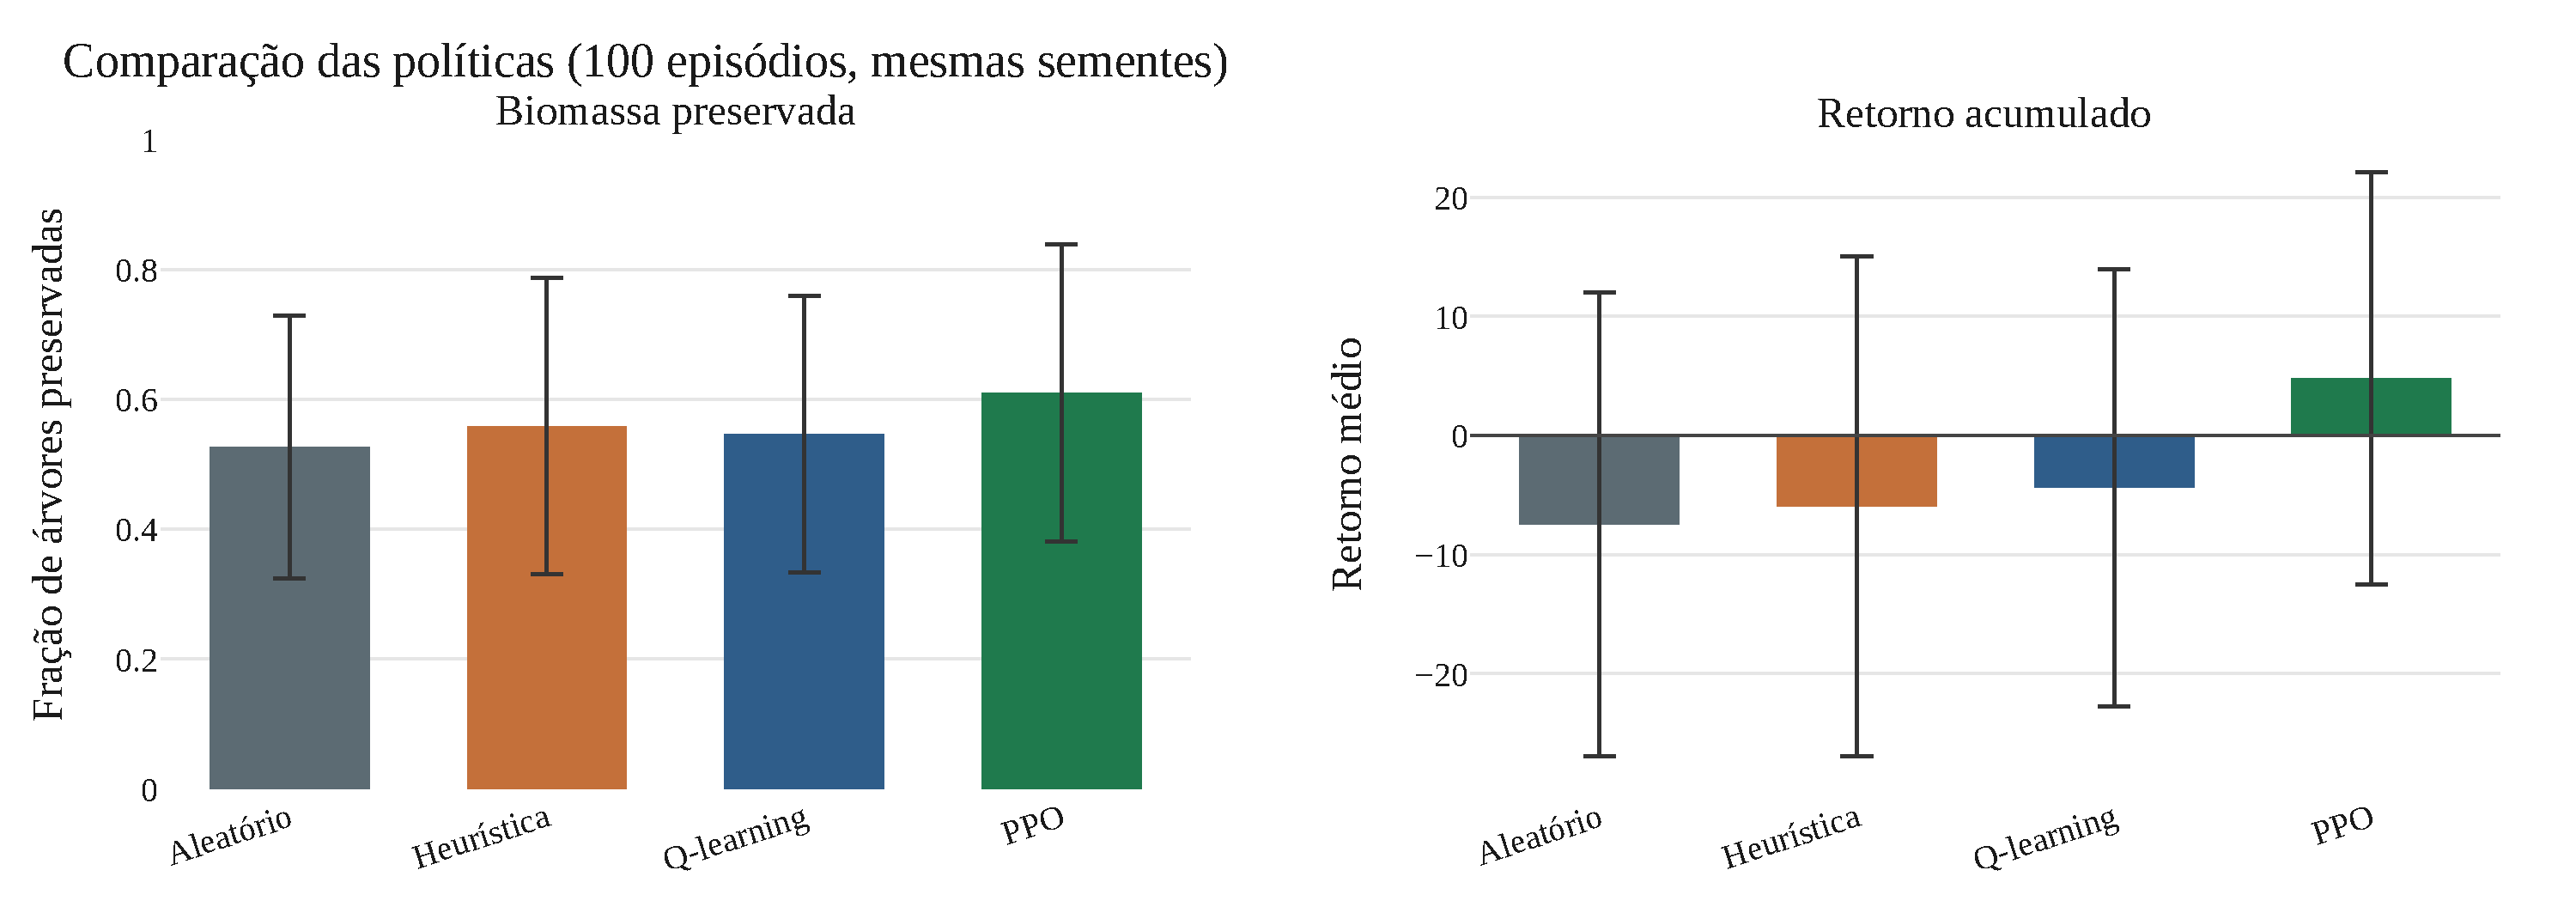
\includegraphics[width=0.92\textwidth]{figures/fig_policy_comparison.pdf}
\caption{Comparação das quatro políticas em 100 episódios de teste.
À esquerda, fração média de árvores preservadas.
À direita, retorno acumulado médio.
As barras de erro representam o desvio padrão.}
\label{fig:bars}
\end{figure}

O fato de o \emph{Q-learning} tabular não superar a heurística é informativo.
Com apenas o índice do centroide e dois bins globais, a tabela $Q$ não
dispõe de graus de liberdade para distinguir configurações em que o risco
está a sotavento.
Nessas condições, a regra fixa ``sempre no centroide'' já é uma boa
aproximação do que o tabular consegue representar, e o custo da exploração
durante o treino não se traduz em ganho claro na avaliação gulosa.

\subsection{Distribuição entre episódios}

A Figura~\ref{fig:violin} mostra a distribuição completa da biomassa
preservada.
Há sobreposição entre políticas, o que é esperado: a configuração inicial dos
três focos domina parte da variância (desvios padrão próximos de $0{,}22$).
Ainda assim, a massa de probabilidade do PPO desloca-se para valores mais
altos, e a mediana acompanha o deslocamento da média.
Isso indica ganho sistemático, e não apenas um ou dois episódios outliers.

\begin{figure}[!ht]
\centering
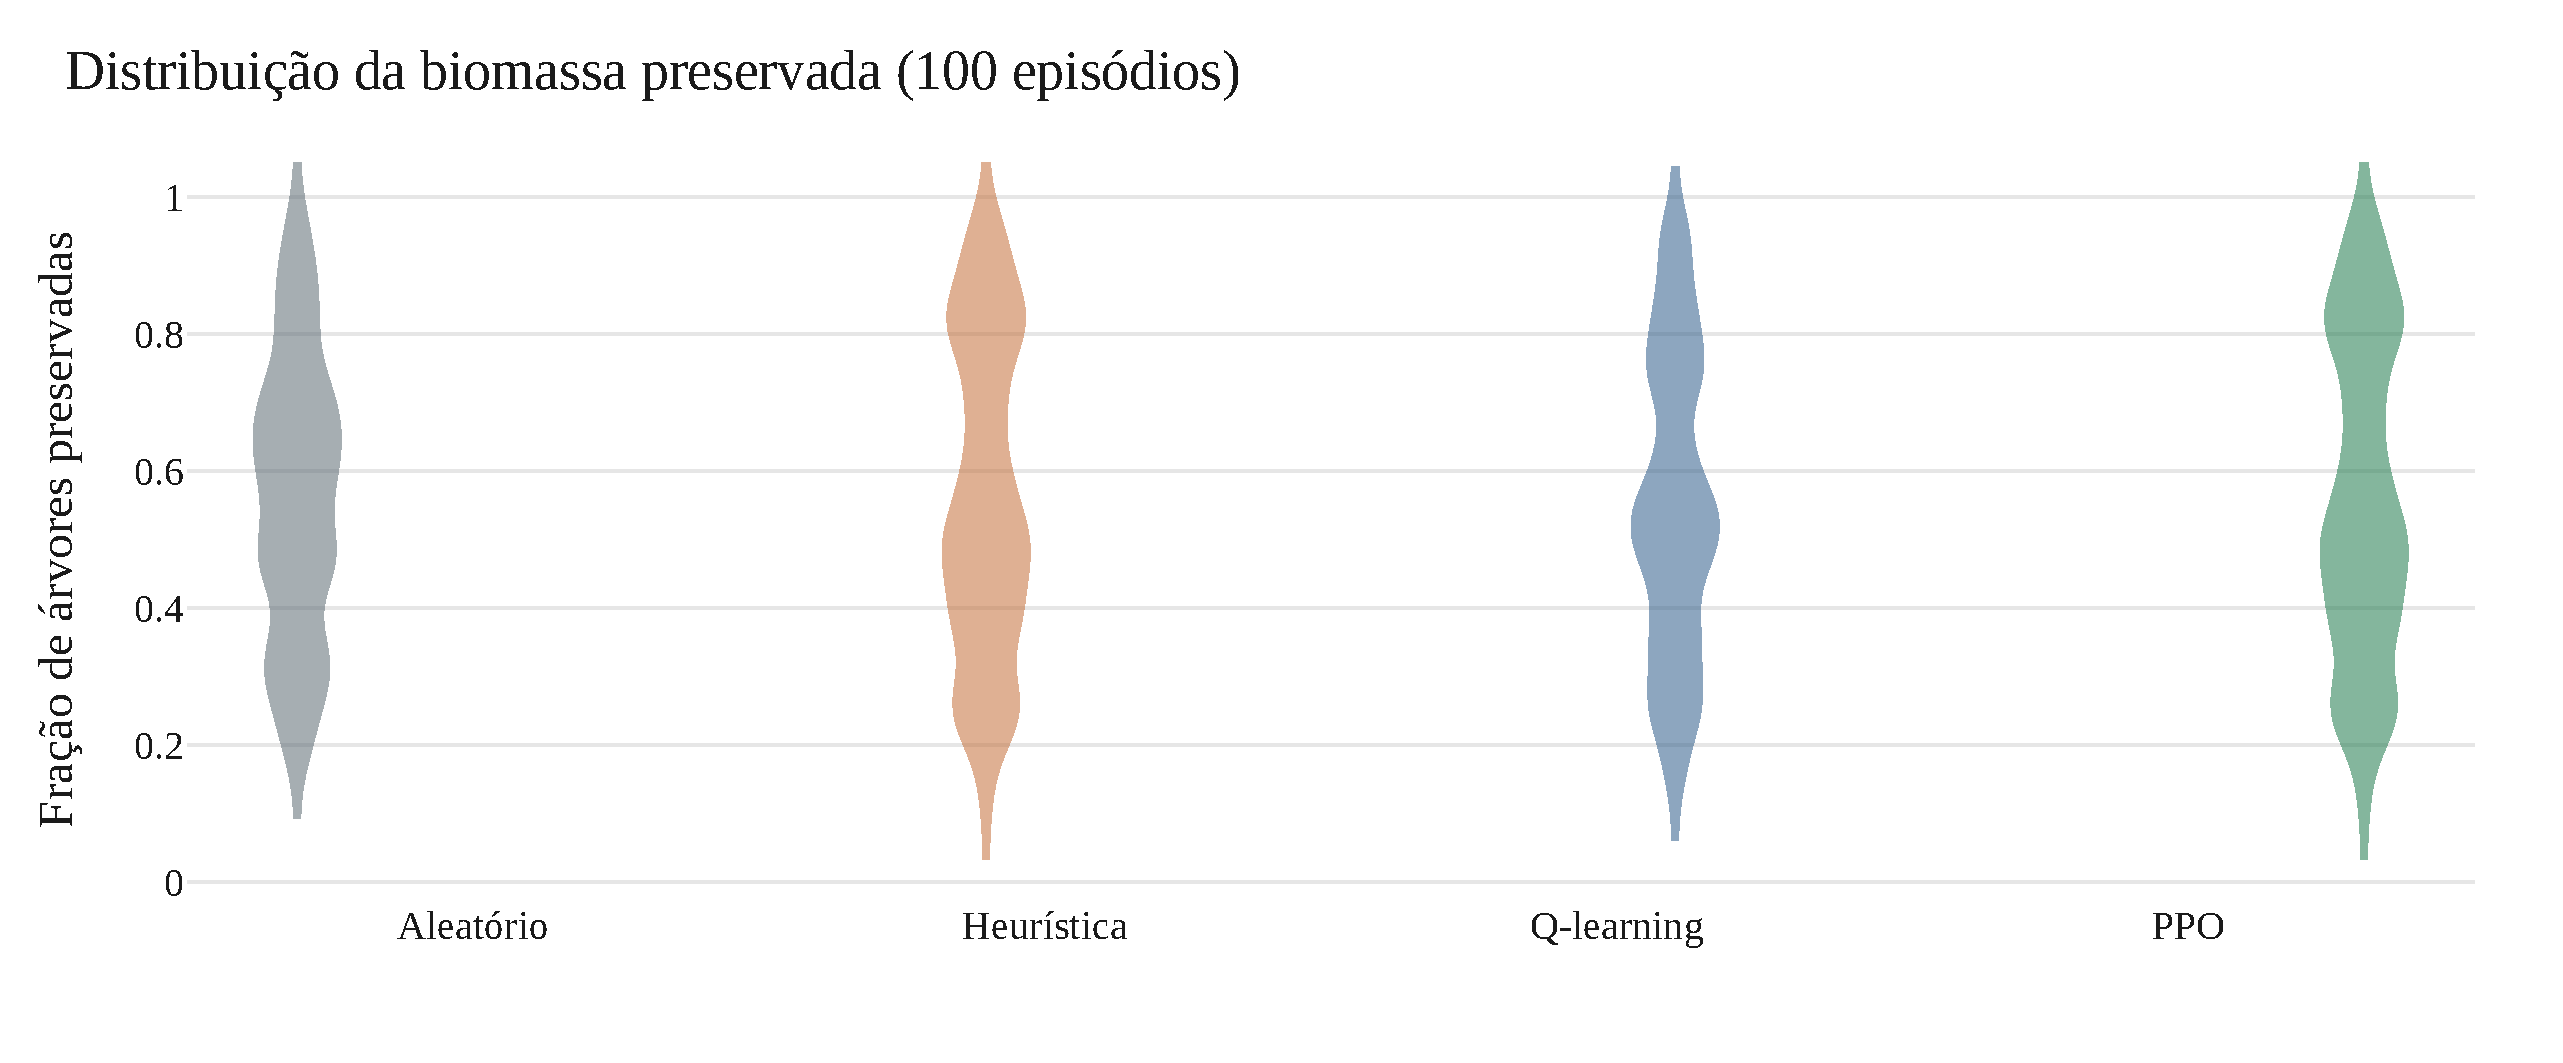
\includegraphics[width=0.75\textwidth]{figures/fig_violin_saved.pdf}
\caption{Distribuição da fração de árvores preservadas em 100 episódios com
sementes compartilhadas.
Violinos com caixa interna e linha de média.}
\label{fig:violin}
\end{figure}

\subsection{Evolução do aprendizado}

A Figura~\ref{fig:learn} apresenta as curvas de retorno durante o treino.
No \emph{Q-learning}, a média móvel sobe rapidamente nas primeiras centenas de
episódios e depois estabiliza em patamar próximo do desempenho da heurística,
coerente com a limitação da observação compacta.
No PPO, o retorno por episódio é ruidoso (como é típico em RL com episódios
curtos e alta variância de mapa), mas a média móvel ascende e atinge valores
positivos nos episódios finais registrados (média dos últimos 50 episódios de
treino aproximadamente $+12$), alinhada ao resultado de teste.

\begin{figure}[!ht]
\centering
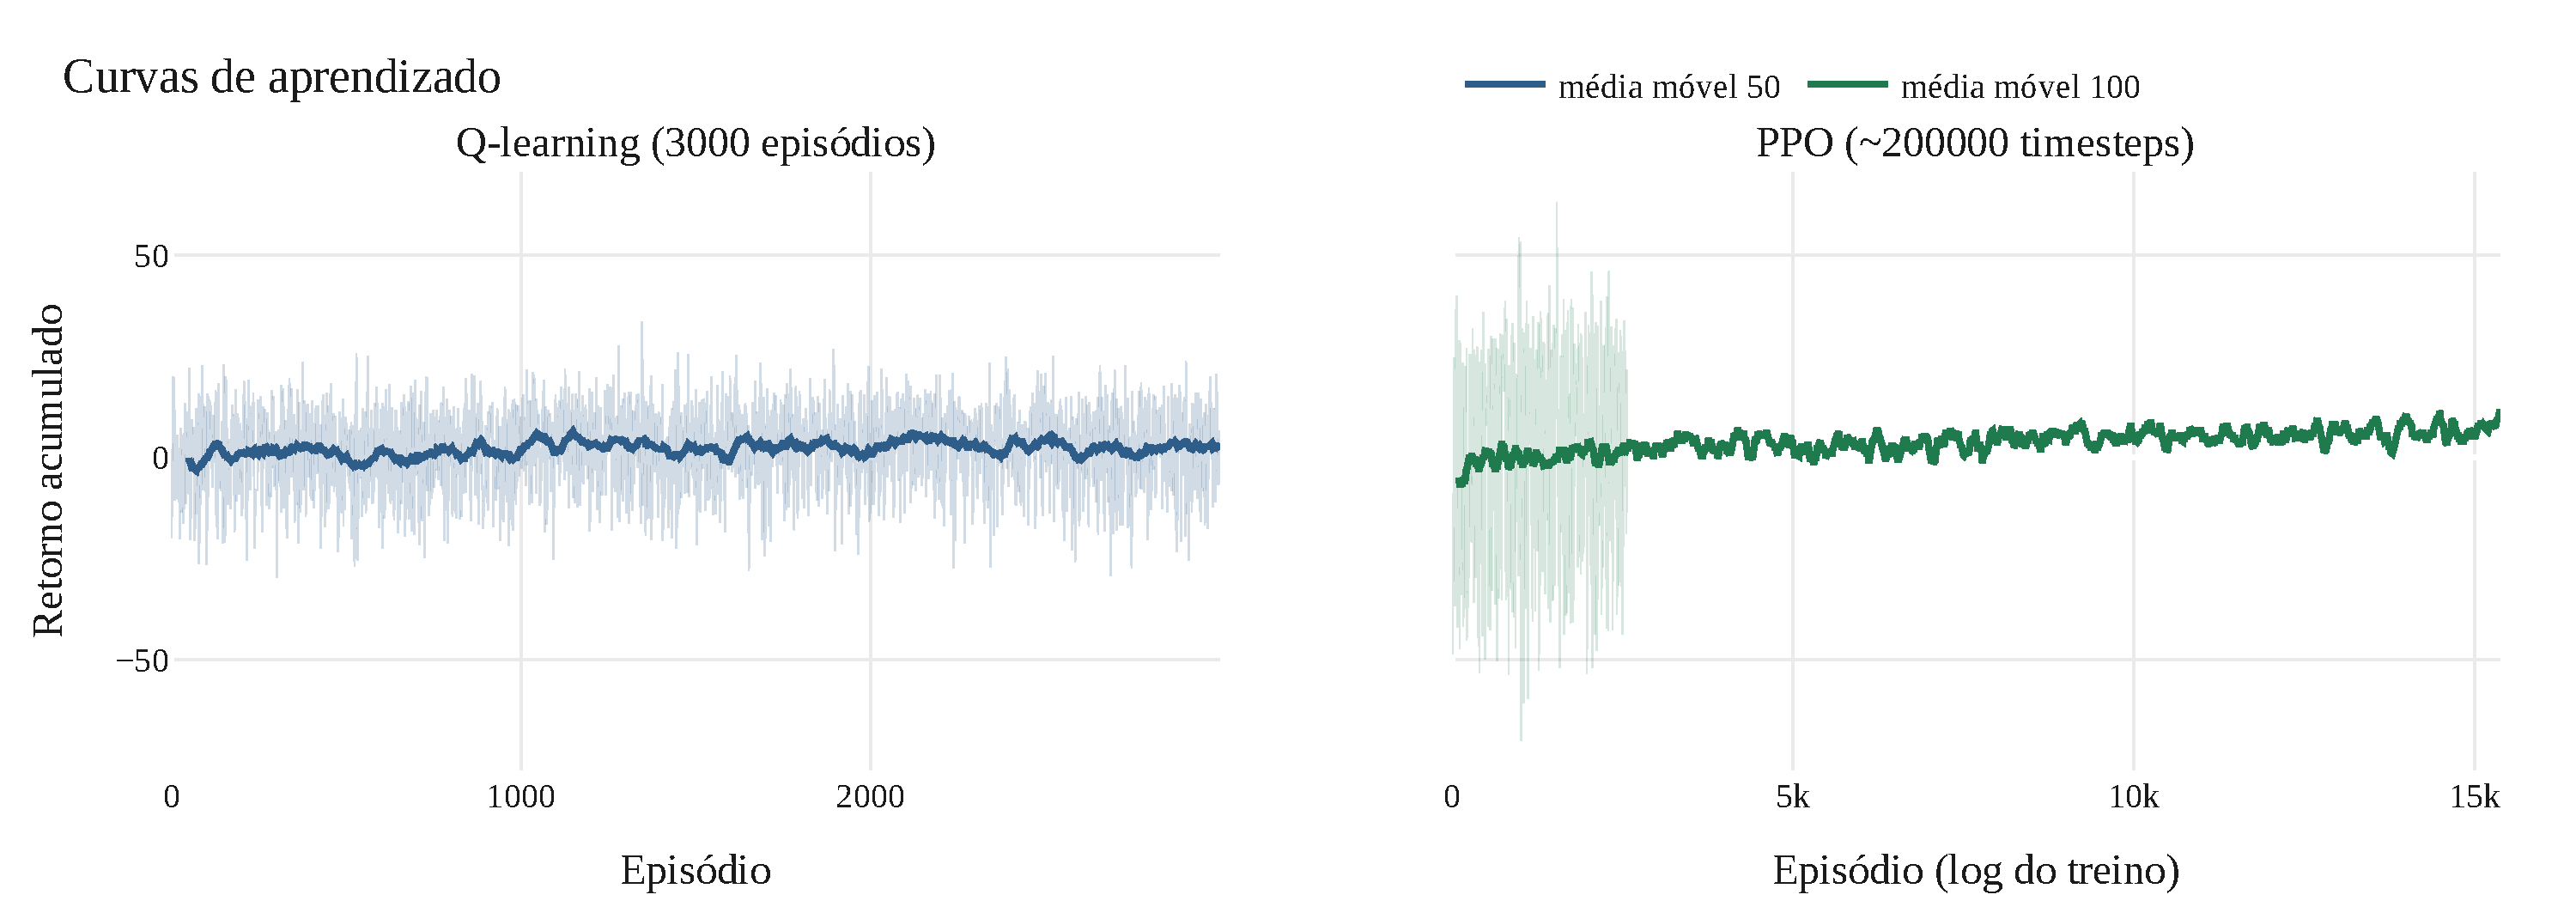
\includegraphics[width=0.92\textwidth]{figures/fig_learning_curves.pdf}
\caption{Curvas de aprendizado do retorno acumulado.
À esquerda, \emph{Q-learning} ao longo de 3000 episódios.
À direita, PPO ao longo dos episódios registrados durante cerca de
$200\,000$ passos de ambiente.
Linhas claras: retorno por episódio.
Linhas escuras: médias móveis.}
\label{fig:learn}
\end{figure}

\subsection{Ilustração espacial do controle}

Para tornar concreta a diferença de estratégia, a Figura~\ref{fig:3d}
exibe o estado final do mesmo mapa inicial (semente $340$) sob quatro
controles, além do estado inicial comum.
Sem controle e sob a heurística, a maior parte da biomassa é consumida
(cerca de \SI{10}{\percent} e \SI{12}{\percent} preservados, respectivamente).
O \emph{Q-learning} melhora parcialmente.
O PPO preserva aproximadamente \SI{91}{\percent} das árvores nesse episódio.
O contraste é mais extremo do que a média da Tabela~\ref{tab:results}, o que
é desejável para ilustração: mostra um regime em que antecipar o sotavento
muda o desfecho qualitativo do incêndio.
A visualização 3D (volumes de copa, chamas e tocos sobre fundo escuro)
documenta o estado da grade após a interação entre o AC e cada política.

\begin{figure}[!ht]
\centering
\begin{subfigure}[t]{0.48\textwidth}
  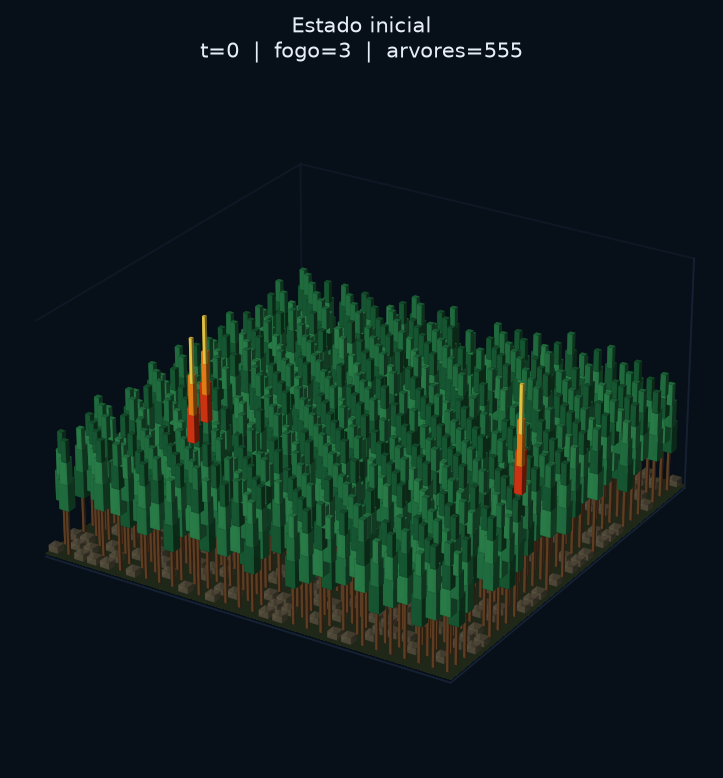
\includegraphics[width=\linewidth]{figures/fig3d_t0.png}
  \caption{Estado inicial (semente 340)}
\end{subfigure}\hfill
\begin{subfigure}[t]{0.48\textwidth}
  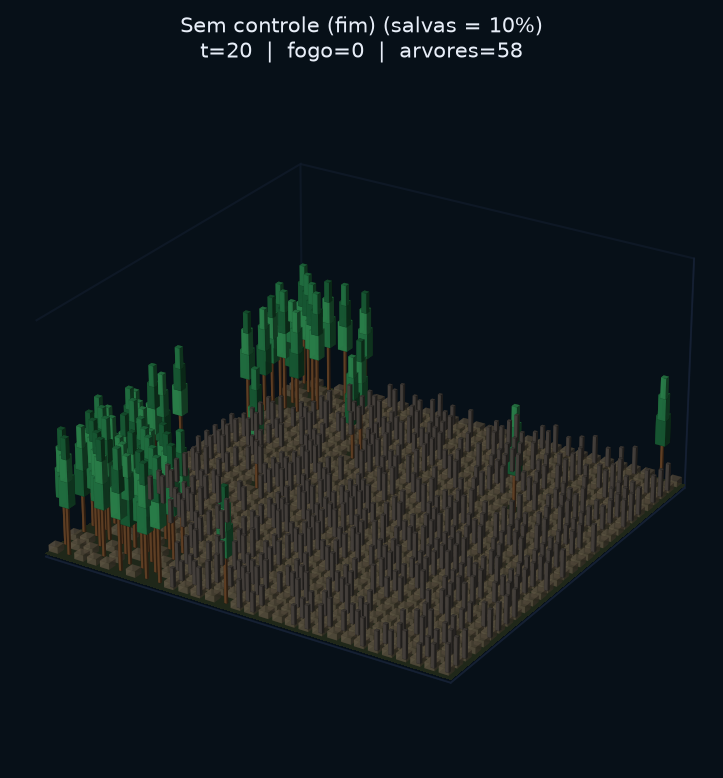
\includegraphics[width=\linewidth]{figures/fig3d_wild_tf.png}
  \caption{Sem controle}
\end{subfigure}

\vspace{0.35em}

\begin{subfigure}[t]{0.32\textwidth}
  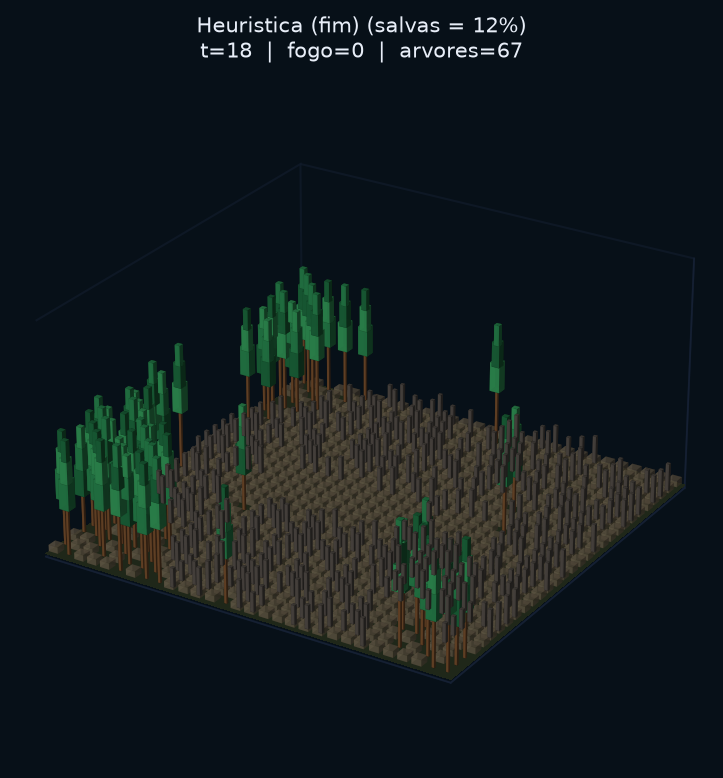
\includegraphics[width=\linewidth]{figures/fig3d_heu_tf.png}
  \caption{Heurística}
\end{subfigure}\hfill
\begin{subfigure}[t]{0.32\textwidth}
  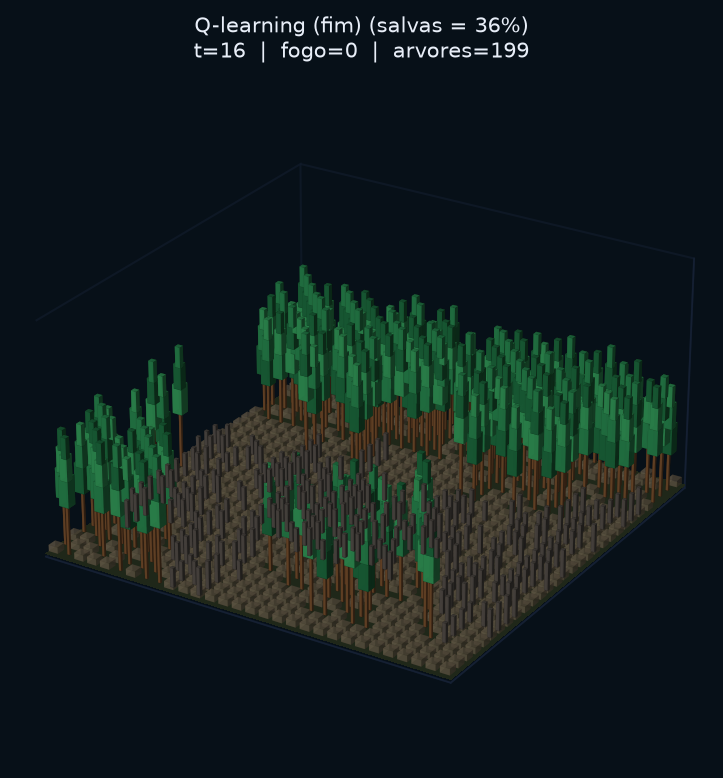
\includegraphics[width=\linewidth]{figures/fig3d_ql_tf.png}
  \caption{Q-learning}
\end{subfigure}\hfill
\begin{subfigure}[t]{0.32\textwidth}
  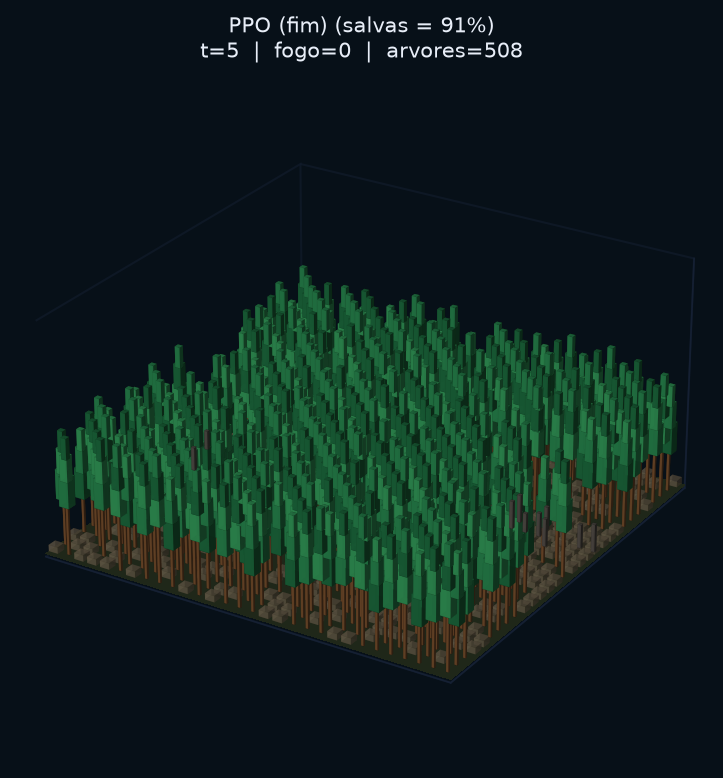
\includegraphics[width=\linewidth]{figures/fig3d_ppo_tf.png}
  \caption{PPO}
\end{subfigure}
\caption{Renderização 3D do desenvolvimento de um episódio ilustrativo
(semente $340$).
Painel (a): configuração inicial compartilhada.
Painéis (b) a (e): estado final sob cada forma de controle.
A mesma física de vento e brasas atua em todos os casos.}
\label{fig:3d}
\end{figure}

\section{Discussão}
\label{sec:discussao}

Os resultados sustentam a tese de que a diferença observada não nasce do
ambiente (fixo e compartilhado), e sim da informação disponível para decidir.
Com vento e brasas, a política eficaz precisa colocar combustível removido
onde o fogo \emph{estará}, não apenas onde ele está.
A heurística e o \emph{Q-learning} compacto operam essencialmente sobre o
centroide; o PPO, ao receber densidades regionais, consegue formar uma
política condicionada à geometria a sotavento.

Esse padrão ilustra um princípio clássico de RL: a representação do estado
limita o desempenho tanto quanto o algoritmo de atualização~\cite{sutton2018}.
Um \emph{Q-learning} com a mesma observação de $77$ dimensões exigiria
discretização agressiva ou aproximação de função, o que o aproximaria, na
prática, de métodos \emph{deep} como o PPO.
A comparação justa que adotamos (mesmo ambiente, mesmas sementes, mesmo
espaço de ações) isola precisamente esse eixo observação versus algoritmo.

\subsection{Limitações}
\label{sec:limitacoes}

A grade é moderada ($30\times 30$); o vento é constante; não há regeneração de
vegetação nem fogo subterrâneo.
A variância entre episódios permanece alta porque a geometria dos três focos
iniciais muda o grau de dificuldade.
A vantagem média do PPO em biomassa é modesta em pontos percentuais, embora
consistente e acompanhada de ganho claro em retorno.
Essas ressalvas não anulam o resultado central: sob física com brasas, a
observação espacial estruturada altera o teto de desempenho.

Em síntese, implementamos um autômato celular de incêndio com vento e brasas e
comparamos, sob protocolo experimental único, quatro formas de abrir aceiros.
O PPO com observação espacial estruturada superou a heurística de centroide, o
\emph{Q-learning} tabular e a política aleatória tanto em biomassa preservada
quanto em retorno.
Além do ranking empírico, a contribuição conceitual é mais ampla: os resultados
sugerem que, em problemas de controle espacial com propagação não local,
investir em representações de estado mais informativas pode ser tão ou mais
importante do que substituir o algoritmo de aprendizado.
No presente estudo, essa ideia aparece na comparação entre uma observação
compacta centrada no centroide e uma observação espacial estruturada capaz de
antecipar risco a sotavento, sem alterar o ambiente físico compartilhado pelas
políticas.

Como extensão natural, a inclusão de fogo subterrâneo (turfa ou húmus que
rebrota após aparente extinção) aumentaria a demanda por antecipação e
memória, ampliando ainda mais o espaço em que políticas com representação espacial
estruturada devem se destacar.

\FloatBarrier
\section{Métodos}
\label{sec:metodos}

\subsection{Autômato celular de incêndio com vento e brasas}
\label{sec:ca}

A floresta é representada por uma grade quadrada de lado $n=30$.
Cada célula assume um entre quatro estados: vazio, árvore, em chamas ou
queimado.
A atualização usa a vizinhança de Moore (oito vizinhos).
No início de cada episódio, as árvores são colocadas com densidade $0{,}60$ e
são acesos três focos independentes.
A probabilidade base de inflamação por contato é
$p_{\mathrm{spread}}=0{,}90$.

A cada passo temporal ocorrem, nesta ordem, três processos:

\begin{enumerate}
  \item Toda célula \emph{em chamas} torna-se \emph{queimada}.
  \item Uma célula \emph{árvore} pode inflamar-se se houver vizinho em chamas.
        A probabilidade de inflamação é maior na direção do vento (aqui o
        vetor constante $(0,+1)$, sentido leste, com fator de reforço
        $2{,}0$) e menor a barlavento.
        Assim, a frente avança preferencialmente a sotavento, o que reproduz a
        assimetria observada em incêndios reais.
  \item Com probabilidade $0{,}28$, cada célula em chamas lança uma brasa que
        pousa entre $3$ e $6$ células a favor do vento, com pequeno desvio
        lateral.
        Se o destino contém uma árvore, esta pode inflamar-se mesmo que haja
        aceiro entre a origem e o destino.
        Esse acoplamento não local é o mecanismo que torna insuficiente a
        mera proteção do centroide atual.
\end{enumerate}

O horizonte máximo de simulação é de $70$ passos; o episódio termina antes
desse limite quando não resta nenhuma célula em chamas.

\subsection{Formulação como processo de decisão de Markov}
\label{sec:mdp}

O controle é modelado como um MDP compatível com a interface
Gymnasium~\cite{towers2023}.
Em cada passo, o agente escolhe onde abrir um aceiro (remoção de combustível)
e, em seguida, o autômato avança um passo.

O espaço de ações é discreto e relativo ao centroide do fogo.
A grade é particionada em uma malha grossa $5\times 5$.
O agente seleciona um dos nove deslocamentos dessa malha em relação à região
que contém o centroide (incluindo o próprio centroide), ou a ação nula
(\emph{no-op}).
Em cada ação efetiva, no máximo oito células de combustível são removidas
dentro da região escolhida.
Essa formulação relativa evita que o agente memorize coordenadas absolutas e
concentra o problema na decisão espacial em torno do foco ativo.

A função de recompensa é deliberadamente neutra quanto à direção do vento.
Ela combina: (i)~um termo positivo proporcional à biomassa ainda viva;
(ii)~penalidade por novas células queimadas; (iii)~bônus por células em chamas
apagadas pelo aceiro; (iv)~custo leve por cortar
árvore verde; (v)~no término, bônus pela fração de árvores preservadas e
penalidade pela área queimada.
Não existe termo que favoreça explicitamente ações a leste.
Qualquer política que se antecipe a sotavento precisa descobrir essa
estratégia a partir da dinâmica observada.

\textbf{Protocolo de comparação justa.}
O ambiente físico (vento, brasas, densidade, orçamento de aceiro) é idêntico
para todas as políticas.
Na avaliação, as sementes aleatórias também são as mesmas.
Portanto, diferenças de desempenho atribuem-se apenas ao algoritmo e à
observação utilizada para decidir.

\subsection{Políticas comparadas}
\label{sec:politicas}

Comparamos quatro agentes que compartilham o mesmo espaço de ações, mas
diferem na forma de escolher a ação e na informação de estado disponível.

\paragraph{Política aleatória.}
Em cada passo, a ação é sorteada de modo uniforme entre as dez opções
(nove deslocamentos relativos e \emph{no-op}).
Esse baseline quantifica o desempenho esperado na ausência de qualquer
conhecimento da dinâmica do fogo.
Como o orçamento de aceiro é limitado, ações aleatórias ocasionalmente
interrompem focos, porém não organizam uma linha de defesa coerente.

\paragraph{Heurística de centroide.}
Enquanto houver células em chamas, a heurística sempre escolhe a ação
relativa $0$, isto é, abre aceiro na região que contém o centroide do fogo.
Se o fogo se extinguiu, escolhe \emph{no-op}.
A regra é transparente e não requer treino: concentra o esforço onde a massa
de fogo está agora.
Sob propagação puramente local, essa estratégia é razoável.
Com vento e brasas, porém, o centroide atrasa o risco verdadeiro, que se
desloca a sotavento e pode ultrapassar a própria barreira que a heurística acaba
de abrir.

\paragraph{\emph{Q-learning} tabular (observação compacta).}
O agente tabular recebe um vetor de observação de baixa dimensão composto por
três inteiros: o índice da região grossa que contém o centroide do fogo, um
nível discretizado da quantidade de fogo e um nível discretizado da quantidade
de árvores restantes.
Com malha $5\times 5$ e cinco níveis discretizados para a intensidade de fogo e
cinco para a biomassa restante, o espaço
de estados contém $625$ entradas.
A tabela $Q(s,a)$ é atualizada pela regra clássica de
Watkins~\cite{sutton2018}, com taxa de aprendizado $\alpha=0{,}25$, fator de
desconto $\gamma=0{,}95$ e exploração $\varepsilon$-greedy decaindo até o piso
$0{,}02$.
O treino durou $3000$ episódios.
Essa representação é suficiente para localizar o centroide e estimar a
severidade global, mas não distingue densidades de combustível ou de fogo em
regiões vizinhas.
Em particular, o agente não ``vê'' um bolsão de árvores a leste do foco, onde
as brasas tendem a cair.

\paragraph{PPO com observação espacial estruturada.}
O PPO~\cite{schulman2017} recebe um vetor contínuo de $77$ dimensões:
três mapas $5\times 5$ com a densidade regional de células em chamas, de
árvores e de células queimadas, concatenados às coordenadas normalizadas do
centroide.
Essa observação preserva a geometria do problema e permite correlacionar a
direção do vento com padrões de risco adiante da frente de fogo.
A política e o crítico são redes MLP treinadas com a implementação
Stable-Baselines3~\cite{raffin2021}, usando $\gamma=0{,}95$, taxa de
aprendizado $3\times 10^{-4}$, clipping $0{,}2$ e $200\,000$ passos de
interação com o ambiente.
Como a observação já carrega a geometria regional do estado, o agente pode, em
princípio, aprender a abrir aceiros \emph{à frente} do centroide, e não
apenas sobre ele.

Em resumo: aleatório e heurística não aprendem; o \emph{Q-learning} aprende
sobre um resumo limitado do estado; o PPO aprende sobre um mapa de densidades.
O ambiente permanece fixo. O que muda é a informação e o método de decisão.

\subsection{Métricas e protocolo de avaliação}
\label{sec:avaliacao}

Avaliamos cada política em $100$ episódios de teste com sementes
$1000,\ldots,1099$, comuns a todos os métodos.
As métricas principais são:
\begin{itemize}
  \item a fração de árvores preservadas ao fim do episódio (biomassa relativa
        à quantidade inicial);
  \item o retorno acumulado (soma das recompensas ao longo do episódio).
\end{itemize}
Reportamos média e desvio padrão.
Para visualizar a variabilidade entre focos iniciais, também examinamos a
distribuição empírica da biomassa preservada.
As curvas de aprendizado usam o retorno por episódio durante o treino do
\emph{Q-learning} e do PPO.
Um episódio ilustrativo com semente $340$ é renderizado em perspectiva 3D
para contrastar o estado final sob diferentes controles.


\section*{Disponibilidade de dados}

O código-fonte, as métricas numéricas, as figuras e as animações 3D deste
estudo estão no repositório do projeto acadêmico.
Os prompts empregados na assistência por inteligência artificial encontram-se
na pasta de documentação do repositório.


\begin{thebibliography}{9}

\bibitem{schiff2008}
J.~L. Schiff.
\newblock \emph{Cellular Automata: A Discrete View of the World}.
\newblock Wiley, 2008.

\bibitem{drossel1992}
B.~Drossel and F.~Schwabl.
\newblock Self-organized critical forest-fire model.
\newblock \emph{Phys.\ Rev.\ Lett.} \textbf{69}, 1629--1632 (1992).

\bibitem{towers2023}
M.~Towers et~al.
\newblock Gymnasium: A standard interface for reinforcement learning
  environments.
\newblock \url{https://gymnasium.farama.org/} (2023).

\bibitem{sutton2018}
R.~S. Sutton and A.~G. Barto.
\newblock \emph{Reinforcement Learning: An Introduction}.
\newblock 2nd~ed. MIT Press, 2018.

\bibitem{schulman2017}
J.~Schulman, F.~Wolski, P.~Dhariwal, A.~Radford and O.~Klimov.
\newblock Proximal Policy Optimization Algorithms.
\newblock arXiv:1707.06347 (2017).

\bibitem{raffin2021}
A.~Raffin, A.~Hill, A.~Gleave, A.~Kanervisto, M.~Ernestus and N.~Dormann.
\newblock Stable-Baselines3: Reliable reinforcement learning
  implementations.
\newblock \emph{J.\ Mach.\ Learn.\ Res.} \textbf{22}(268), 1--8 (2021).

\end{thebibliography}

\end{document}

